%; whizzy chapter
% -initex iniptex -latex platex -format platex -bibtex jbibtex -fmt fmt
% $B0J>e(B whizzytex $B$r;HMQ$9$k>l9g$N@_Dj!#(B


%     Tokyo Debian Meeting resources
%     Copyright (C) 2008 Junichi Uekawa

%     This program is free software; you can redistribute it and/or modify
%     it under the terms of the GNU General Public License as published by
%     the Free Software Foundation; either version 2 of the License, or
%     (at your option) any later version.

%     This program is distributed in the hope that it will be useful,
%     but WITHOUT ANY WARRANTY; without even the implied warranty of
%     MERCHANTABILITY or FITNESS FOR A PARTICULAR PURPOSE.  See the
%     GNU General Public License for more details.

%     You should have received a copy of the GNU General Public License
%     along with this program; if not, write to the Free Software
%     Foundation, Inc., 51 Franklin St, Fifth Floor, Boston, MA  02110-1301 USA

%  preview (shell-command (concat "evince " (replace-regexp-in-string "tex$" "pdf"(buffer-file-name)) "&"))
% $B2hA|%U%!%$%k$r=hM}$9$k$?$a$K$O(Bebb$B$rMxMQ$7$F(Bboundingbox$B$r:n@.!#(B
%(shell-command "cd image200804; ebb *.png")

%%$B$3$3$+$i%X%C%@3+;O!#(B

\documentclass[mingoth,a4paper]{jsarticle}
\usepackage{monthlyreport}
\usepackage[dvips]{xy}

% $BF|IU$rDj5A$9$k!"Kh7nJQ$o$j$^$9!#(B
\newcommand{\debmtgyear}{2008}
\newcommand{\debmtgmonth}{4}
\newcommand{\debmtgdate}{19}
\newcommand{\debmtgnumber}{39}

\begin{document}

\begin{titlepage}
\thispagestyle{empty}

% $B%?%$%H%k%Z!<%8(B:$BJT=8I,MW$JItJ,$O:G=i$N%^%/%m$KHt$P$9$3$H(B

\vspace*{-2cm}
$BBh(B\debmtgnumber{}$B2s(B $BEl5~%(%j%"(B Debian $BJY6/2q;qNA(B

\hspace*{-2.4cm}
\includegraphics[width=210mm]{image200801/2008title.eps}\\
\hfill{}\debmtgyear{}$BG/(B\debmtgmonth{}$B7n(B\debmtgdate{}$BF|(B

\end{titlepage}

\dancersection{Introduction}{$B>e@n(B $B=c0l(B}
 
 $B:#7n$N(BDebian$BJY6/2q$X$h$&$3$=!#$3$l$+$i(BDebian$B$N@$3&$K$"$7$rF'$_F~$l$k$H(B
 $B$$$&J}$b!"$9$G$K$I$C$W$j$H$D$+$C$F$$$k$H$$$&J}$b!"7n$K0l2s(BDebian$B$K$D$$(B
 $B$F8l$j$^$;$s$+!)(B

 Debian$BJY6/2q$NL\E*$O2<5-$G$9!#(B

\begin{itemize}
 \item \underline{Debian Developer} ($B3+H/<T(B)$B$N0i@.!#(B
 \item $BF|K\8l$G$N!V(B\underline{$B3+H/$K4X$9$k>pJs(B}$B!W$r@0M}$7$F$^$H$a!"%"%C%W%G!<%H$9$k!#(B
 \item \underline{$B>l(B}$B$NDs6!!#(B
 \begin{itemize}
  \item $BIaCJ$P$i$P$i$J>l=j$K$$$k?M!9$,(B face-to-face $B$G=P2q$($k>l$rDs6!(B
	$B$9$k!#(B
  \item Debian $B$N$?$a$K$J$k$3$H$r8l$k>l$rDs6!$9$k!#(B
  \item Debian$B$K$D$$$F8l$k>l$rDs6!$9$k!#(B
 \end{itemize}
\end{itemize}		

 Debian$B$NJY6/2q$H$$$&$3$H$G5f6KE*$K$O;22C<TA40w$,(BDebian Package$B$r$,$j$,$j(B
 $B$H:n$k%9!<%Q!<%O%C%+!<$K$J$C$?;Q$rLQA[$7$F$$$^$9!#>pJs$N6&M-!&3hMQ$rDL$7(B
 $B$F(B Debian$B$N:#8e$NG=F0E*$JE83+$X$NEZBf$H$7$F!"!V>l!W$H$7$F$N6u4V$rDs6!$9(B
 $B$k$N$,L\E*$G$9!#(B

$B0J>e$rL\E*$H$7$?!"(B2008 $BG/%"%8%'%s%@$G$9!'(B
\begin{enumerate}
 \item $B?7G/2q!V5$9g$rF~$l$k!W(B
 \item Open Source Conference Tokyo (3/1)
 \item $B%G!<%?$@$1$N%Q%C%1!<%8$r:n@.$7$F$_$k!"(B
       $B%i%$%;%s%9$N9M$(J}(B (David Smith)
 \item $B%P%$%J%j0l$D$N%Q%C%1!<%8$r:n@.$7$F$_$k(B ($B5HED(B@$BHD66(B)\\
       $B%P!<%8%g%s4IM}%D!<%k$r;H$$(BDebian$B%Q%C%1!<%8$r4IM}$9$k(B(git)\\
       $B%"%C%W%9%H%j!<%`$N07$$(B(svn/git/cvs)($B4d>>(B $B?.MN$5$s(B)
 \item $B%P%$%J%j$NJ,$1$?%Q%C%1!<%8$N:n@.!#(B($BA0ED$5$s(B)\\
       $B%P%$%J%j$NJ,$1J}$N9M$(J}!"%"%C%W%0%l!<%I$J$I$N1?MQ$H$+!#(B
 \item $B%Q%C%1!<%8:n@.(B(dpatch/debhelper$B$G:n@.$9$k%Q%C%1!<%8(B)($B>.NS576)$5$s(B)\\
       man $B$N=q$-J}(B(roff or docbook)($B$G$s$5$s(B)
 \item $B%Q%C%1!<%8:n@.(B(kernel patch$B!"(Bkernel module)
       $B!"(BDebconf$BH/I=N}=,(B
 \item Debconf $B%"%k%<%s%A%s!"6&M-%i%$%V%i%j%Q%C%1!<%8:n@.(B

 \item Open Source Conference Tokyo/Fall$B!"(B
       $B%G!<%b%s7O$N%Q%C%1!<%8$N:n@.!"(Blatex$B!"(B emacs-lisp$B!"%U%)%s%H%Q%C%1!<%8(B
 \item $B%Q%C%1!<%8$N(B cross-compile $B$NJ}K!!"(Bamd64 $B>e$G(B i386 $B$N%Q%C%1!<%8$H(B
       $B$+!"(BOSC-Fall$BJs9p2q!"(BDebconf$BJs9p2q(B
 \item $B9q:]2=(B po-debconf / po$B2=(B / DDTP
 \item $BK:G/2q(B
\end{enumerate}


\newpage

\begin{minipage}[b]{0.2\hsize}
 \definecolor{titleback}{gray}{0.9}
 \colorbox{titleback}{\rotatebox{90}{\fontsize{80}{80} {\gt $B%G%S%"%sJY6/2q(B} }}
\end{minipage}
\begin{minipage}[b]{0.8\hsize}
\hrule
\vspace{2mm}
\hrule
\tableofcontents
\vspace{2mm}
\hrule
\end{minipage}

\dancersection{$B;vA02]Bj(B}{$B>e@n(B $B=c0l(B}

$B:#2s$N;vA02]Bj$O0J2<$G$9!#(B

\begin{enumerate}
 \item ...

\end{enumerate}

$B$3$N2]Bj$KBP$7$FDs=P$$$?$@$$$?FbMF$O0J2<$G$9!#(B


%%% trivia quiz
\dancersection{Debian Trivia Quiz}{$B>e@n(B $B=c0l(B}

$B$H$3$m$G!"$_$J$5$s(B Debian $B4XO"$NOCBj$K$*$$$D$$$F$$$^$9$+!)(BDebian$B4XO"$NOC(B
$BBj$O%a!<%j%s%0%j%9%H$r$h$s$G$$$k$HDI@W$G$-$^$9!#$?$@$h$s$G$$$k$@$1$G$O$O(B
$B$j$"$$$,$J$$$N$G!"M}2rEY$N%F%9%H$r$7$^$9!#FC$K0l?M$@$1$G$O0UL#$,$o$+$i$J(B
$B$$$H$3$m$b$"$k$+$bCN$l$^$;$s!#$_$s$J$G0l=o$KFI$s$G$_$^$7$g$&!#(B

$B:#2s$N=PBjHO0O$O(B\url{debian-devel-announce@lists.deban.org} $B$KEj9F$5$l$?(B
$BFbMF$+$i$G$9!#(B
\begin{multicols}{2}
 
 \santaku
 {}
 {}
 {}
 {}
 {}

\end{multicols}

\dancersection{$B:G6a$N(BDebian$B4XO"$N%_!<%F%#%s%0Js9p(B}{$B>e@n(B $B=c0l(B}
\subsection{$BEl5~%(%j%"(BDebian$BJY6/2q(B38$B2sL\Js9p(B}

% (query-replace-regexp "<.*?>" "")
% (query-replace-regexp "^[	 ]\+" "")

3$B7n$KBh(B38$B2sEl5~%(%j%"(BDebian$BJY6/2q$r<B;\$7$^$7$?!#(B
$B:#2s$N;22C<T$O(B
$B>.NS$5$s!"$"$1$I$5$s!"(BHenrich$B$5$s!"A0ED$5$s!";3K\9@G7$5$s!"KYFb$5$s!"(Bhisashim$B$5$s!"(B
$B;T@n7{?M$5$s!"2-Cf8&?4$5$s!"(BDavid Smith$B$5$s!"4X:,Bn$5$s!"(Bgotom$B$5$s!"(B
$BLnB<$5$s!";3:,=S><$5$s!"(Bsatoken$B$5$s!"(Bosamu matsumoto$B$5$s!"(B
osamu kimura $B$5$s!"%-%?%O%i$5$s!"@DLZ=$$5$s!"(BIan $B$5$s!"(B
$B5HED!wHD66$5$s!"4X:,!w(BGoogle$B$5$s!"(Bjitsukata$B$5$s!"(B
Noriaki Sato$B$5$s!"$9$:$-$/$K$*$5$s!"F#:j$5$s!"(B
CCG$B$5$s!"86ED$5$s!"F|HfLn7<$5$s!"$G$s$9$1!wAjLO86$5$s!"(B
$B_@Ln$5$s!"1|LnM35*$5$s!"%7$5$s!"9b66$5$s!"(B
Emmet Hikory$B!"1-;tJ8IR$5$s!"(B
$B>e@n$N(B37$B?M$G$7$?!#(B

$B$^$:!"%/%$%:$r:#2s$b<B;\$7$^$7$?!#(B
$B:#2s$b!"(Bdebian-devel-announce $B$NFbMF$+$i=PBj$7$^$7$?!#(B
7$BLdL\$^$G$GA40wIT@52r$K$J$C$?$N$G!"(B8$BLdL\$GGT<TI|3h$7$?$H$3$m!"(B
$B$d$^$M$5$s$,:G8e$^$G>!$A;D$j$^$7$?!#$*$a$G$H$&$4$6$$$^$9!#(B

3$B7n(B1$BF|$K3+:E$5$l$?(BOpen Source Conference $B;22C$K$D$$$F;3:,$5$s$,Js9p$7$^$7$?!#(B

2008$BG/$O%F!<%^$H$7$F(BDEB$B%Q%C%1!<%8$N3+H/!&4IM}$K4XO"$7$?FbMF$K$7$h$&!"$H$$$&$3$H$K$7$F$$$?$N$G(B
$B:#2s$O:G=i$N%F!<%^$H$7$F!"%G!<%?%Q%C%1!<%8$NOC$r$7$^$7$?!#(B
David Smith$B$,H/I=$7$^$7$?!#(B
CDBS$B$r;H$C$?>l9g$K4JC1$K%Q%C%1!<%8$,:n@.$G$-$k$H$$$&N.$l$G$N@bL@$G$7$?!#(B

Debian$B%Q%C%1!<%8$G$N%i%$%;%s%9$N<h07$$$K$D$$$F>R2p$7$^$7$?!#(B
$B%i%$%;%s%9$rD4$Y$F%Q%C%1!<%8$G(Bdebian/copyright$B$r:n@.$9$k>l9g$N0lHLE*$J<j=g$r>R2p$7$^$7$?!#(B

$B:#2s$O1c2q$O(B
$B!V0C(BGuRi$B!J$"$0$j!K(B 5566$B!W(B
$B$K$F3+:E$7$^$7$?!#(B


\dancersection{$B%P%$%J%j0l$D$@$1$N%Q%C%1!<%8$r:n@.$7$F$_$k(B}{$B5HED!wHD66(B}
\label{sec:binpkg}
\index{XX@YY} 

\dancersection{$B%P!<%8%g%s4IM}%D!<%k$r;H$$(B Debian $B%Q%C%1!<%8$r4IM}$9$k(B Git$BJT(B}{$B4d>>(B $B?.MN(B}
\label{sec:vcsgit}
\index{XX@YY} 

\subsection{$B$O$8$a$K(B}
$B:G6a$N(B Debian Package $B$O!"(BVCS\footnote{Version Control System}$B$r;H$C$F4IM}$9$k(B
$B$3$H$,$G$-$k$h$&$K$J$C$F$*$j!"<B:]$KMxMQ$7$F$$$k%a%s%F%J$bB?$/$J$j$^$7$?!#(B
VCS$B$H8@$C$F$bMM!9$G$9$,!"(BDebian $B$G$OBeI=E*$J(BVCS$B$G$"$k(B CVS, Subversion $B$d(B $B:G6aN.9T$j$N(B Git$B!"(B
$B%^%$%J!<$J(B VCS$B$G$"$k(B darcs $B$J$I$r;H$&$3$H$,$G$-$^$9!#(B
$B:#2s$O!":#0lHV%$%1$F$$$k$H;W$o$l$k(B Git $B$r;H$$!"(BDebian Package $B$r%P!<%8%g%s4IM}$9$k$3$H$K$h$j$I$N$h$&(B
$B$JMxE@$,$"$k$N$+!"$I$N$h$&$J%D!<%k$r;H$C$F%a%s%F%J%s%9$r9T$($P$$$$$N$+!"$J$I$K$D$$$F$r@bL@$7$^$9!#(B

\subsection{$B%=!<%9%Q%C%1!<%8$r!!(BGit $B$G4IM}$9$k$?$a$N%D!<%k(B}
Debian $B%Q%C%1!<%8$r(B Git $B$G4IM}$9$k$?$a$N%D!<%k$H$7$F!"(B git-buildpackage $B$,$"$j$^$9!#(B
$B$3$l$r;H$&$3$H$K$h$C$F!"(BGit $B$r;H$C$F%Q%C%1!<%8$N%=!<%9%3!<%I$r4IM}$9$k$3$H$,$G$-$k$h$&$K$J$j$^$9!#(B
$B%$%s%9%H!<%k$O$$$D$b$N$H$*$j!"(B{\bf apt-get} or {\bf aputitude} $B$G!#(B

\begin{commandline}
$sudo  apt-get install git-buildpackage
\end{commandline}

\subsubsection{git-buildpackage$B$GDs6!$5$l$k%3%^%s%I(B}
git-buildpackage$B$GDs6!$5$l$k%3%^%s%I$O0J2<(B4$B$D$7$+$"$j$^$;$s!#(B
$B$3$l$i$N%3%^%s%I$H%*%W%7%g%s$r;H$C$F!"%Q%C%1!<%8$N%a%s%F%J%s%9$r$9$k$3$H$K$J$j$^$9!#(B

   \begin{table}[h]
    \begin{center}
      {
        \begin{tabular}{l|l} \hline
                $BDs6!$5$l$k%3%^%s%I(B & $B5!G=(B \\ \hline \hline
/usr/bin/git-buildpackage & $B%Q%C%1!<%8$r:n@.$9$k(B \\
/usr/bin/git-dch & Git $B$N%3%_%C%H%m%0$+$i(B Debian Changelog $B$r:n@.$9$k!#(B\\
/usr/bin/git-import-dsc & $B4{B8$N(B Debian Package $B$r(BGit$B$K%$%s%]!<%H$9$k!#(B\\
/usr/bin/git-import-orig & $B%"%C%W%9%H%j!<%`$+$i%j%j!<%9$5$l$?%=!<%9%3!<%I$r(BGit$B$K%$%s%]!<%H$9$k!#(B\\
           \end{tabular}
        }
     \caption{git-buildpackage $B$GDs6!$5$l$k%3%^%s%I(B}
     \label{git-buildpackage-command}
    \end{center}
    \end{table}

\subsection{git-buildpackage $B$r;H$$4IM}$7$F$_$k(B}
Debian $B%Q%C%1!<%8$K$O(B2$B$D$N>uBV$,$"$k$H9M$($i$l$^$9!#0l$D$O4{$K%Q%C%1!<%82=$5$l$F$$$k$b$N!#(B
$B$b$&$R$H$D$O!":#$+$i(BDebian $B%Q%C%1!<%8$K$7$h$&$H$7$F$$$k$b$N$G$9!#(B
$B$^$:$O!"4{$K(BDebian $B%Q%C%1!<%8$K$J$C$F$$$k$b$N$r(B Git $B$G4IM}$9$kJ}K!$r@bL@$7$^$9!#(B

\subsubsection{$B4{$K%Q%C%1!<%82=$5$l$F$$$k$b$N$r(B Git $B$G4IM}$9$k(B}

$B$^$:!"(Bgit-import-dsc$B%3%^%s%I$r;H$$!"!!(BGit $B%j%]%8%H%j$K8=:_$N%=!<%9%3!<%I$N>uBV$r(B
$B<h$j9~$_$^$9!#%3%^%s%I$N%*%W%7%g%s$K!"%Q%C%1!<%8$N(B dsc$B%U%!%$%k(B\footnote{Debian $B%Q%C%1!<%8$N@)8f%U%!%$%k(B}
$B$r;XDj$7$^$9!#<B9T$9$k$H!"%Q%C%1!<%8L>$G%G%#%l%/%H%j$,:n@.$5$l!"(BGit $B%j%]%8%H%j$,:n@.$5$l$^$9!#(B
$B$^$?!"%V%i%s%A$H$7$F!"(Bmaster $B%V%i%s%A$H!"(Bupstream $B%V%i%s%A$,:n@.$5$l$^$9!#!!(BDebain $B4X78$N%3!<%I$O(B
 master 
$B%V%i%s%A!"(BUpstream $B$N%=!<%9%3!<%I$O(B upstream $B%V%i%s%A$G4IM}$5$l$k$h$&$K$J$j$^$9(B\footnote{$B%V%i%s%A$O(B git branch $B%3%^%s%I$GI=<(2DG=(B}$B!#(B

\begin{commandline}
$ git-import-dsc ../isight-firmware-tools_1.0.2-1.dsc
Upstream version: 1.0.2
Debian version: 1
No git repository found, creating one.
Initialized empty Git repository in .git/
Everything imported under isight-firmware-tools
$ ls
isight-firmware-tools
$ cd isight-firmware-tools
$ git branch
* master
  upstream
\end{commandline}

\subsection{$B%$%s%]!<%H;~$N%m%0(B}

$B%Q%C%1!<%8$r%$%s%]!<%H$7$?$H$-$K!"(BGit $B$N%3%_%C%H%m%0$K8=:_$N%P!<%8%g%s$N%3%_%C%H%m%0$,=q$-9~$^$l$^$9!#(B
$B$^$?!"(B Debian Version $B$O(B Git $B$N%?%05!G=$r;H$$!"%?%0L>$H$7$FJ]B8$5$l$^$9!#(B

\begin{commandline}
$ git log
commit 9c3669a233afe69d7be2aa8ad1995e6b19c841aa
Author: Nobuhiro Iwamatsu <iwamatsu@nigauri.org>
Date:   Sun Apr 6 21:48:40 2008 +0900

    Imported Debian patch 1.0.2-1
$ git tag
debian/1.0.2-1
upstream/1.0.2
\end{commandline}

\subsubsection{$B%=!<%9%3!<%I$rJQ99$7!"=$@5$r4IM}$9$k(B}

$B%=!<%9%3!<%I$r=$@5$7!"(BDebian Package$B!!$GG[I[$9$kItJ,$r4IM}$9$k$K$O!":#$^$G$I$*$j!"(Bdpatch$B$J$I$N(B
$B%Q%C%A4IM}%7%9%F%`$r;H$&I,MW$,$"$j$^$9!#(B
$B:n@.$7$?%Q%C%A$r%j%]%8%H%j$K%3%_%C%H$9$k;~$K$K!"(B{\bf git add}, {\bf git commit} $B%3%^%s%I$r;H$$!"(B
$B%j%]%8%H%j$KH?1G$5$;$^$9!#(B

\begin{commandline}
$ dpatch-edit-patch 05_change_ift-load_install_dir
... $B$$$m$$$m=$@5(B ...
$ exit
$ vi debian/patches/00list
$ git add debian/patches/05chage_ift-load_install_dir.dpatch
$ git commit -s debian/patches/00list debian/patches/05_chage_ift-load_install_dir.dpatch
/* $B%(%G%#%?$,5/F0$9$k$N$G!"%3%_%C%H%m%0$r5-=R(B */

Change ift-load install dir.
    
Signed-off-by: Nobuhiro Iwamatsu <iwamatsu@nigauri.org>

$ git log
commit c9865153ae1949956fdfe3827c0da9b36c2f0ddb
Author: Nobuhiro Iwamatsu <iwamatsu@nigauri.org>
Date:   Sun Apr 6 21:23:20 2008 +0900

    Change ift-load install dir.
    
    Signed-off-by: Nobuhiro Iwamatsu <iwamatsu@nigauri.org>
\end{commandline}

\subsubsection{git-buildpackage $B$r;H$C$?(BDebian $B%Q%C%1!<%8$N:n@.(B}

Debian $B%Q%C%1!<%8$r:n@.$9$k$K$O!"(B git-buildpackage $B%3%^%s%I$r;H$$$^$9!#(B
--git-ignore-new$B!!%*%W%7%g%s$O!!(BGit $B$KH?1G$5$l$F$$$J$$=$@5$rL5;k$9$k$?$a$N(B
$B%*%W%7%g%s$G$9!#(B
\begin{commandline}
$ git-buildpackage --git-ignore-new -us -uc
\end{commandline}

\subsubsection{$B%Q%C%1!<%8$r%j%j!<%9$9$k(B}
$B?7$7$$(B Debian $B%P!<%8%g%s$N%Q%C%1!<%8$r%j%j!<%9$9$k>l9g$O!"(Bgit-dch $B%3%^%s%I$K(B
--release $B%*%W%7%g%s$rIU$1$^$9!#<B9T$9$k$3$H$K$h$j!"%(%G%#%?$,N)$A>e$,$j!"(BGit
$B$N%3%_%C%H%m%0$+$i!"(BDebian Changelog $B$,:n@.$5$l$^$9!#(B
Changelog $B$r:n@.$7$?$i!"(Bgit-buildpackage $B%3%^%s%I$K(B --git-tag $B%*%W%7%g%s$r(B
$BIU$1$F%Q%C%1!<%8$r:n@.$7$^$9!#(B--git-tag $B$rIU$1$k$H!"%j%]%8%H%j$K(B Debian $B%P!<%8%g%sMQ$N(B
$B%?%0$,:n@.$5$l!"%j%j!<%9$,>pJs$,IU2C$5$l$^$9!#(B
\begin{commandline}
$ git-dch --release
$ git-buildpackage --git-ignore-new --git-tag
$ git tag
debian/1.0.2-1
debian/1.0.2-2
upstream/1.0.2
\end{commandline}

\subsubsection{$B?7$7$$%P!<%8%g%s$K$9$k(B}
$B?7$7$$%P!<%8%g%s$K$9$k$K$O!"(Bgit-import-orig $B%3%^%s%I$r;H$$!"%j%j!<%9$5$l$?(B
$B?7$7$$%P!<%8%g%s$N(B Tar $B%\!<%k$r;XDj$7$^$9!#(B
$B;XDj$9$k$3$H$K$h$j!"%U%!%$%kL>$+$i%P!<%8%g%s$r<hF@$7!"?7$?$K(BUpstream $BMQ$N(B
$B%?%0$,:n@.$5$l$^$9!#(B
$B$^$?!"%"%C%W%9%H%j!<%`$N%P!<%8%g%s$,>e$,$k$?$a!"<+F0E*$K(B Debian Changelog $B$K(B $B<!$N(BDebian Package 
$B%P!<%8%g%s$,DI5-$5$l$^$9!#(B
\begin{commandline}
$ git-import-orig /tmp/isight-firmware-tools-1.2.tar.gz
Upstream version is 1.2.0
Importing '/tmp/isight-firmware-tools-1.2.tar.gz' to branch 'upstream'...
Switched to branch "upstream"
rm 'isight.rules.in'
rm 'po/fr_FR.po'
Created commit f5c85da: Imported Upstream version 1.2.0
 33 files changed, 4434 insertions(+), 1332 deletions(-)

.......<snip>

 src/udev.c                             |  164 +++
 33 files changed, 4434 insertions(+), 1332 deletions(-)
 rename po/{fr_FR.po => fr.po} (66%)
 create mode 100644 src/50-isight-firmware.fdi
 create mode 100644 src/callout.c
 create mode 100644 src/isight-firmware.fdi
 rename isight.rules.in => src/isight.rules.in (100%)
 create mode 100644 src/load.h
 create mode 100644 src/udev.c
Succesfully merged version 1.2 of /home/iwamatsu/Desktop/isight-firmware-tools-1.2.tar.gz into .
$ git branch
debian/1.0.2-1
debian/1.0.2-2
upstream/1.0.2
upstream/1.2
$ cat debian/changelog
isight-firmware-tools (1.2-1) unstable; urgency=low

  * New Upstream Version

 -- Nobuhiro Iwamatsu <iwamatsu@nigauri.org>  Fri, 11 Apr 2008 17:18:23 +0900

\end{commandline}

\subsection{$B?7$?$K%Q%C%1!<%82=$9$k>l9g(B}
$B$"$?$i$7$/$K%=%U%H%&%'%"$r(B Debian Package $B$K$7$F!"!!(Bgit-buildpackage $B$G(B
$B4IM}$9$k>l9g$O(B $B:G=i$K(B Git $B$N5!G=$,I,MW$G$9!#(B
$B$^$:!"%m!<%+%k(B Git $B%j%]%8%H%j$r:n@.$7$^$9!#<!$K:n@.$7$?%j%]%8%H%j$K0\F0$7!"(Bgit-import-orig
$B$K%"%C%W%9%H%j!<%`$N%=!<%9%3!<%I$r;XDj$7!"<B9T$7$^$9!#%=!<%9%3!<%I$O!"(Bgzip$B!"(Bbzip2 $B$J$I$G(B
$B05=L$5$l$?$b$N$H!"E83+$5$l$?%=!<%9%3!<%I%G%#%l%/%H%j$r;XDj$9$k$3$H$,2DG=$G$9!#(B

$B<B9T$9$k:]$K!"(B-u $B%*%W%7%g%s$G!"%"%C%W%9%H%j!<%`$N%P!<%8%g%s$r;XDj$9$kI,MW$,$"$j$^$9!#(B
$B%j%]%8%H%j$r:n@.$7$?8e$O(B upstream $B%V%i%s%A$K0\F0$7!"(B{\bf dh\_make}$BEy$r;H$C$F%Q%C%1!<%8$N?w7A:n@.$7!"(B
$B>e$G@bL@$7$?N.$l$G%a%s%F%J%s%9$r9T$$$^$9!#(B

\begin{commandline}
$ mkdir isight-firmware-loader
$ cd isight-firmware-tools
$ git-init /* $B%m!<%+%k(B Git $B%j%]%8%H%j$r:n@.$9$k(B */
$ git-import-orig -u 1.2 $B!!(B/tmp/isight-firmware-tools-1.2.tar.gz /* $B%=!<%9%3!<%I$r%3%_%C%H(B */
Upstream version is 1.2
Initial import of '/tmp/isight-firmware-tools-1.2.tar.gz' ...
Succesfully merged version 1.2 of /tmp/isight-firmware-tools-1.2.tar.gz into .
$ git log
commit 9bf014aee2f834576f8f03d67ab66e8c85726832
Author: Nobuhiro Iwamatsu <iwamatsu@nigauri.org>
Date:   Tue Apr 8 21:42:55 2008 +0900

    Imported Upstream version 1.2
$ git branch
* master
  upstream
$ git tag
upstream/1.2
$ git branch upsteam
$ dh_make
$ git branch master
\end{commandline}

%\subsubsection{git-buildpackage $B$N@_Dj!!(B.git/gbp.conf}
%git-buildpackage $B$O:Y$+$$@_Dj$r9T$&$3$H$,2DG=$G$9!#(B
%$B@_Dj%U%!%$%k$r(B .git $B%U%!%$%k(B


\dancersection{$B%"%C%W%9%H%j!<%`$N(BVCS$B$HIU$-9g$&(B}{$B4d>>(B}
\label{sec:upstreamvcs}
\index{DebianWithVCS}

CVS / SVN / $B$J$I$N(BVCS$B$r(Bupstream $B$,3hMQ$7$F$$$k>l9g$NOC!#(B

\dancersection{Nexenta Core Platform$B$r;H$C$F$_$k(B}{$B>e@n(B}
\label{sec:nexentacore}
\index{OpenSolaris} 
\index{Nexenta} 


\subsection{$B$O$8$a$K(B}

Nexenta$B$H$O!&!&!&(B

Open Solaris $B$H$O!&!&!&(B

GNU/Linux $B$H$NE}9g$H$O!&!&!&(B


Nexenta Core Platform $B$,(B2$B7n$K%j%j!<%9$5$l$^$7$?!#:#2s$O$=$l$r;n$7$F$_$^(B
$B$9!#(B

\subsection{$B%@%&%s%m!<%I(B}

\url{http://www.nexenta.org/os/DownloadMirrors}$B$+$i%j%s%/$r$?$I$j%@%&%s(B
$B%m!<%I$7$^$9!#(B
$B:#2s$O(B
\url{http://mirror.stanford.edu/nexenta/isos/nexenta-core-platform_1.0-b82_x86.iso.zip}
$B$rMxMQ$7$^$7$?!#(B

unzip$B%3%^%s%I$GE83+$9$k$H(Biso$B%$%a!<%8$,:n@.$5$l$^$9!#(B
\begin{commandline}
[21:54:42]dancer64:nexenta> unzip nexenta-core-platform_1.0-b82_x86.iso.zip 
Archive:  nexenta-core-platform_1.0-b82_x86.iso.zip
  inflating: nexenta-core-platform_1.0-b82_x86.iso  
\end{commandline}

\subsection{Qemu$B4D6-$G$N%$%s%9%H!<%k(B}


$B$^$:!"(Bqemu $BMQ$N%G%#%9%/%$%a!<%8$r:n@.$7$^$9!#(B
\begin{commandline}
[21:55:19]dancer64:nexenta> qemu-img create -f qcow2 nexenta.cow 3GB 
Formatting 'nexenta.cow', fmt=qcow2, size=3145728 kB
\end{commandline}

qemu$B$r5/F0$7$^$9!#(B
\footnote{$B;~4V$N@_Dj$K$D$$$F$O$J$s$H$J$/5sF0$,JQ$G$9!#(BBIOS$B;~4V$r%m!<%+%k%?%$%`$H(B
$B$7$F07$&$o$1$G$b$J$/!"(BUTC$B$H$7$F07$&$o$1$G$b$J$$$_$?$$$G$9!#(B}

\begin{commandline}
[21:55:39]dancer64:nexenta> qemu-system-x86_64 -hda nexenta.cow \
 -cdrom  nexenta-core-platform_1.0-b82_x86.iso \
 -boot d \
 -m 512 
\end{commandline}


$B%a%K%e!<$rA*Br$7=gHV$K%$%s%9%H!<%k:n6H$r?J$a$^$9!#(B

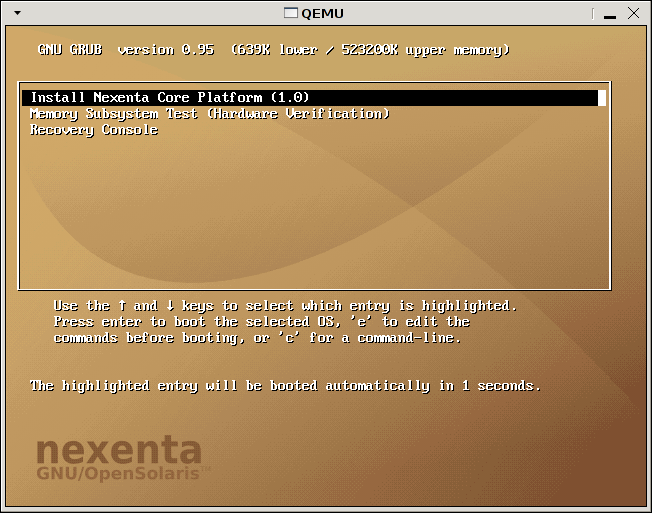
\includegraphics[width=0.5\hsize]{image200804/nexenta1.png}
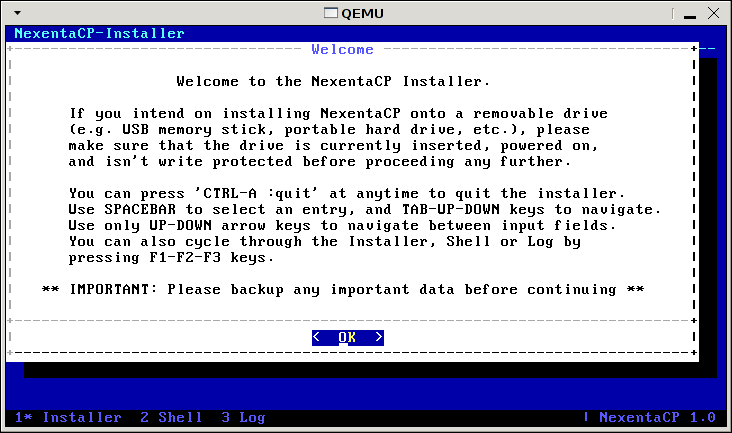
\includegraphics[width=0.5\hsize]{image200804/nexenta2.png}
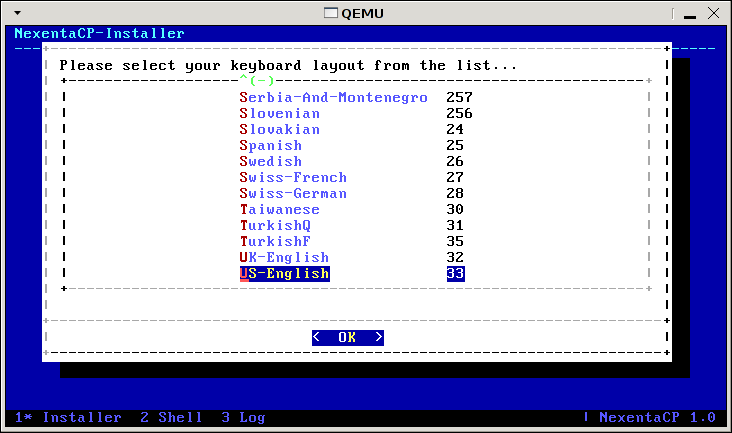
\includegraphics[width=0.5\hsize]{image200804/nexenta3.png}
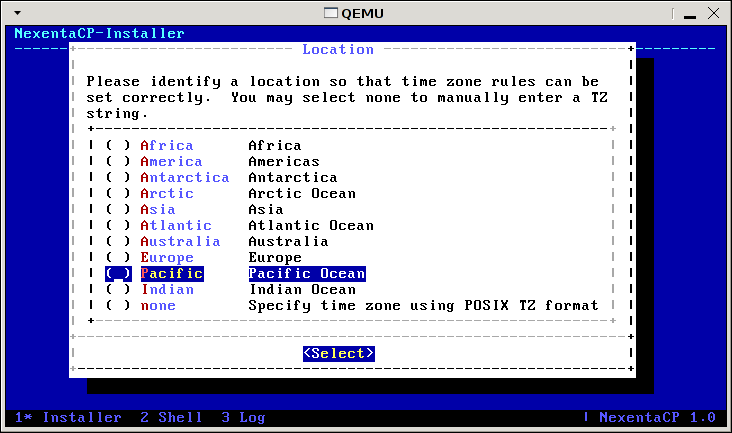
\includegraphics[width=0.5\hsize]{image200804/nexenta4.png}
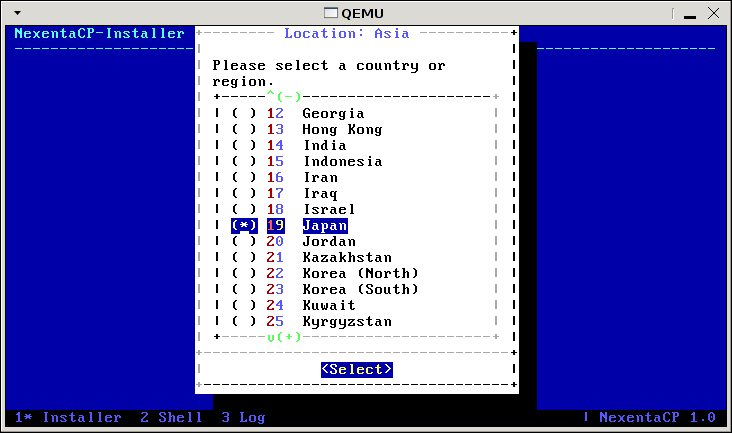
\includegraphics[width=0.5\hsize]{image200804/nexenta5.png}
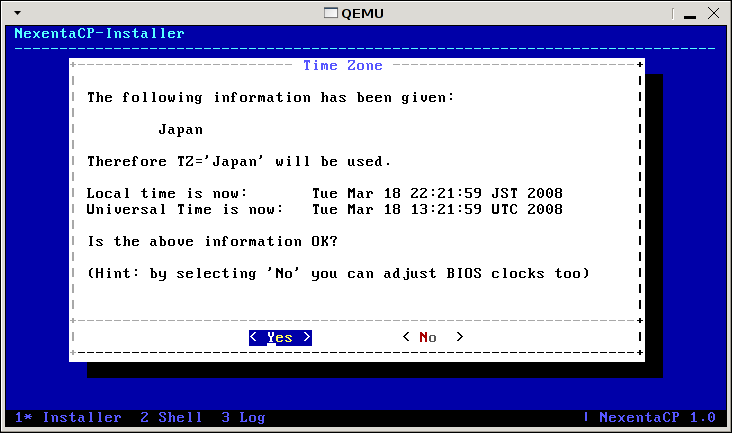
\includegraphics[width=0.5\hsize]{image200804/nexenta6.png}
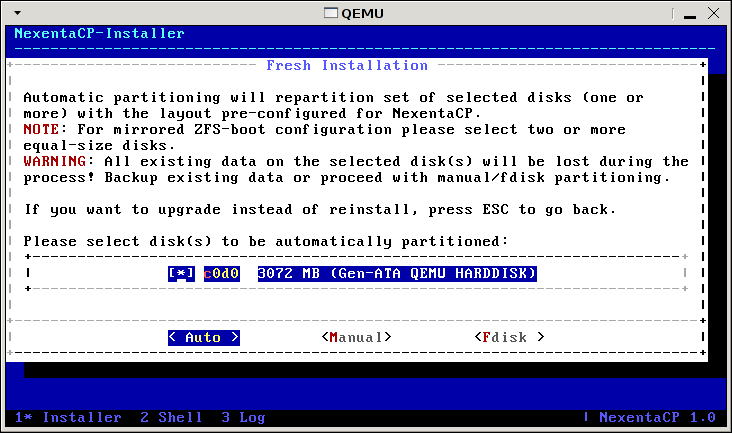
\includegraphics[width=0.5\hsize]{image200804/nexenta7.png}
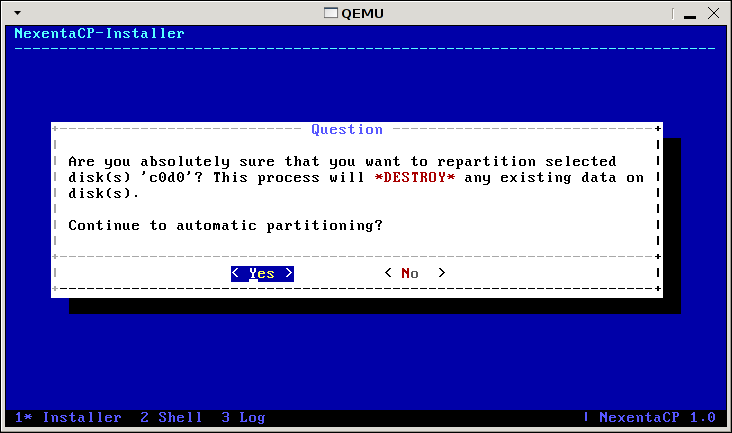
\includegraphics[width=0.5\hsize]{image200804/nexenta8.png}

$B%$%s%9%H!<%k$,3+;O$7$?$i$7$P$7BT$A$^$9!#(B\footnote{AMD Athlon 64 3500+ $B$N(B
$B%^%7%s(B(64bit)$B$G(Bkqemu$B$rMxMQ$7$F(B2$B;~4V$+$+$j$^$7$?(B}

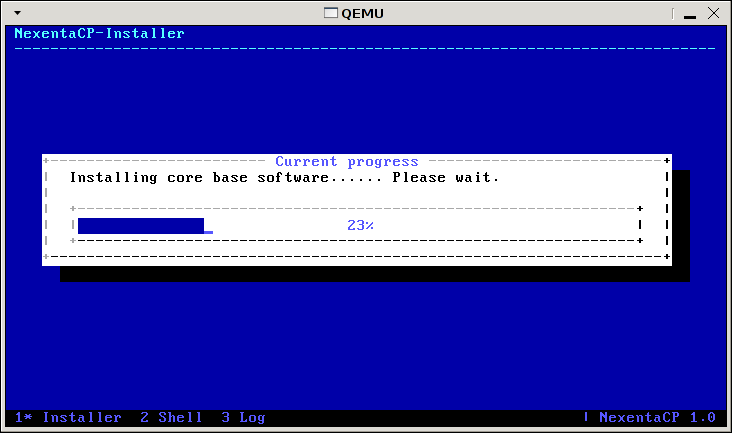
\includegraphics[width=0.5\hsize]{image200804/nexenta9.png}
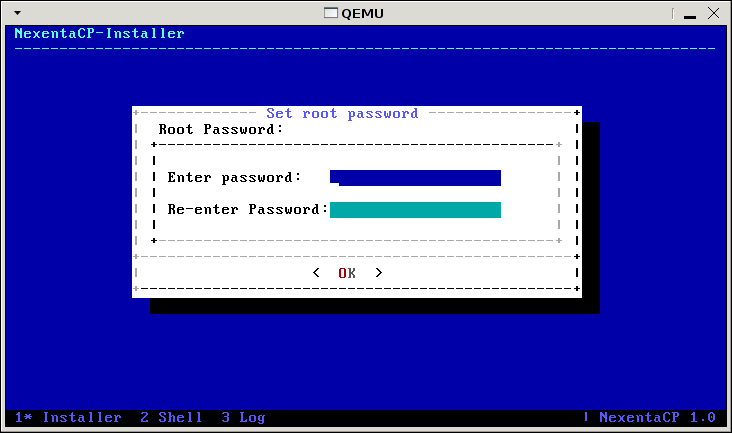
\includegraphics[width=0.5\hsize]{image200804/nexenta10.png}
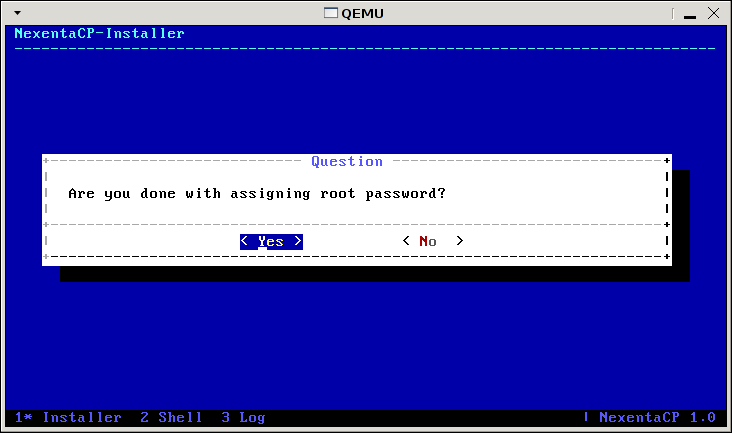
\includegraphics[width=0.5\hsize]{image200804/nexenta11.png}
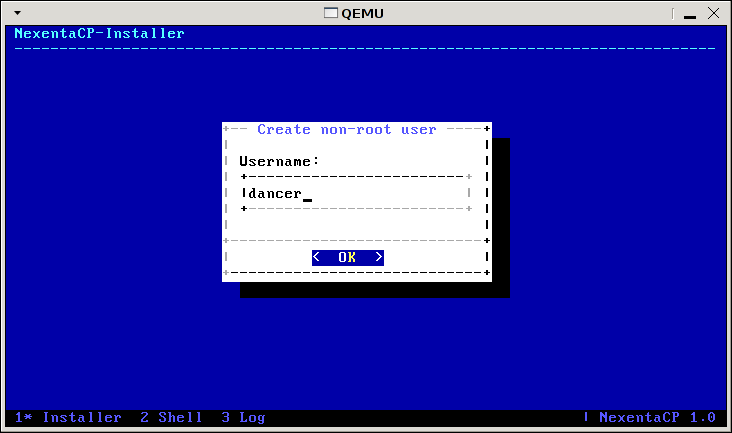
\includegraphics[width=0.5\hsize]{image200804/nexenta12.png}
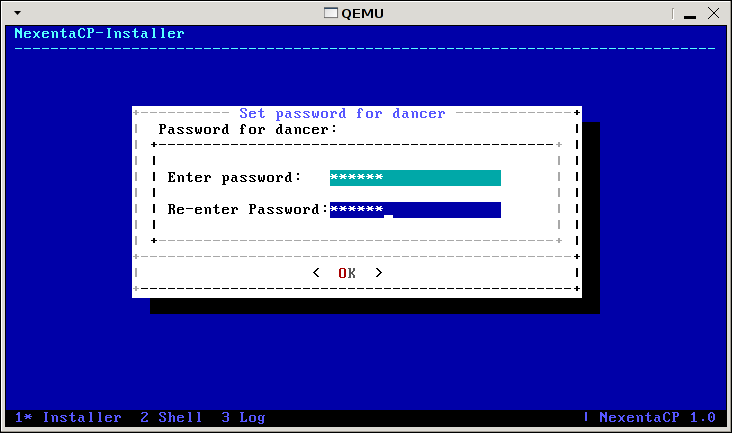
\includegraphics[width=0.5\hsize]{image200804/nexenta13.png}
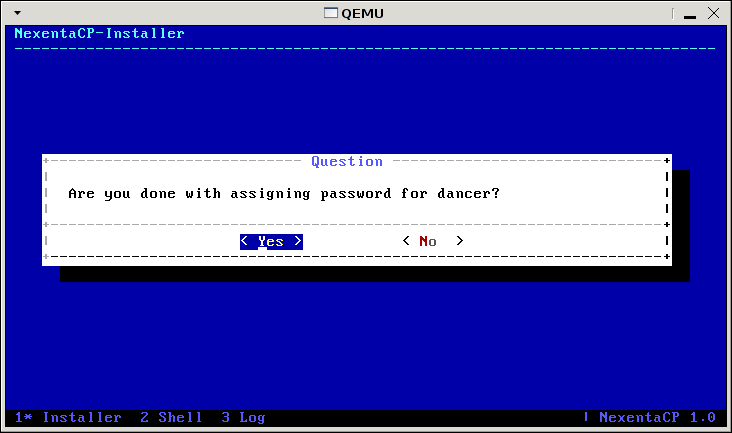
\includegraphics[width=0.5\hsize]{image200804/nexenta14.png}
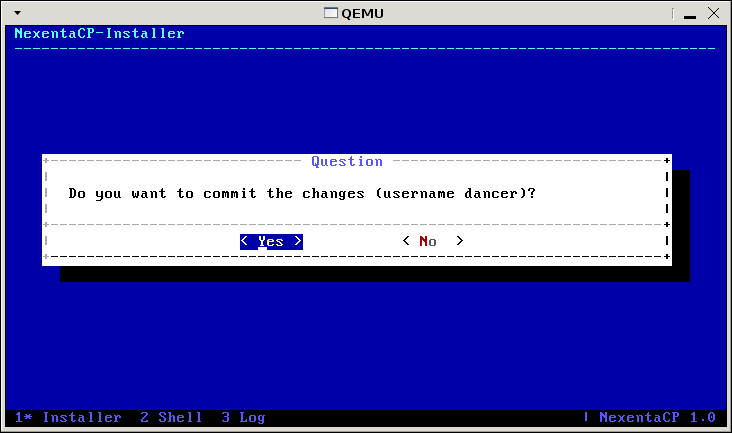
\includegraphics[width=0.5\hsize]{image200804/nexenta15.png}
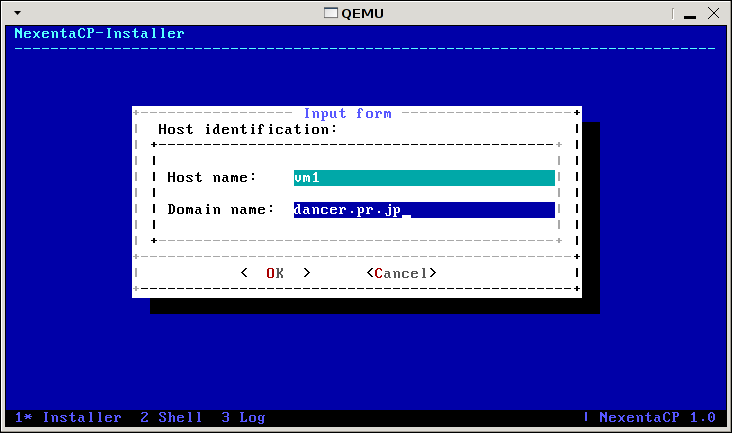
\includegraphics[width=0.5\hsize]{image200804/nexenta16.png}
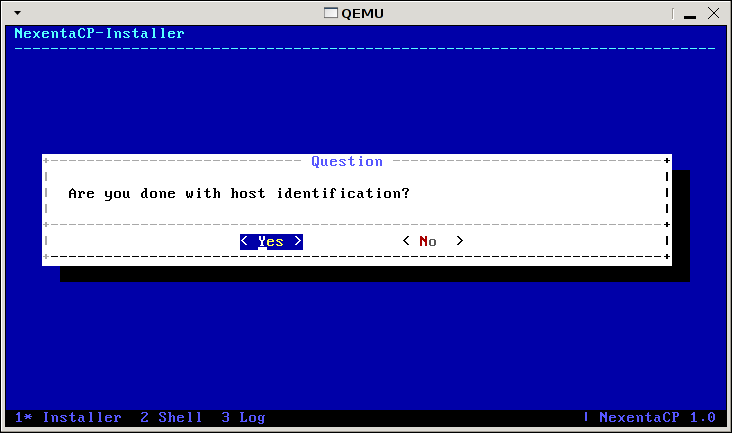
\includegraphics[width=0.5\hsize]{image200804/nexenta17.png}
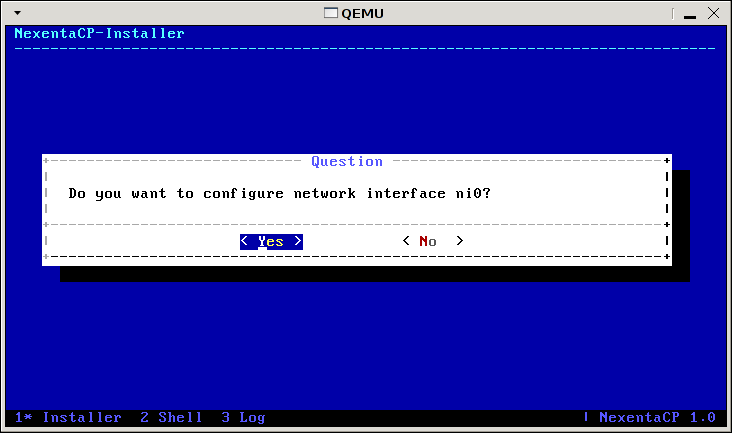
\includegraphics[width=0.5\hsize]{image200804/nexenta18.png}
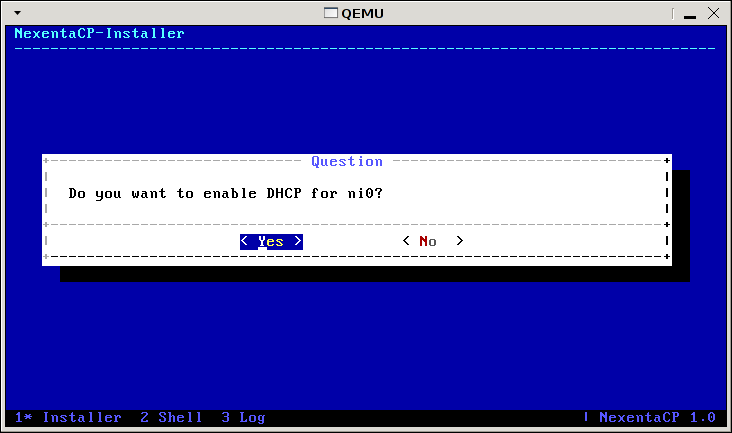
\includegraphics[width=0.5\hsize]{image200804/nexenta19.png}
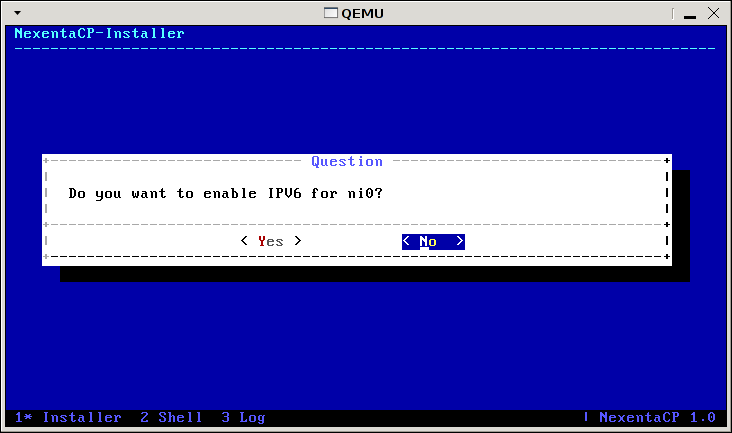
\includegraphics[width=0.5\hsize]{image200804/nexenta20.png}
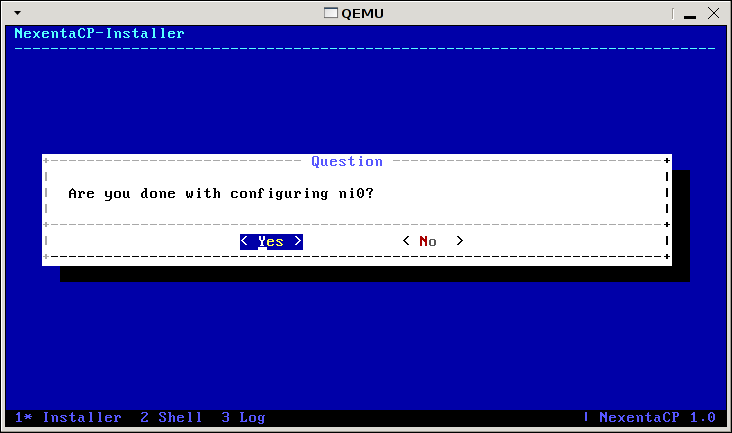
\includegraphics[width=0.5\hsize]{image200804/nexenta21.png}
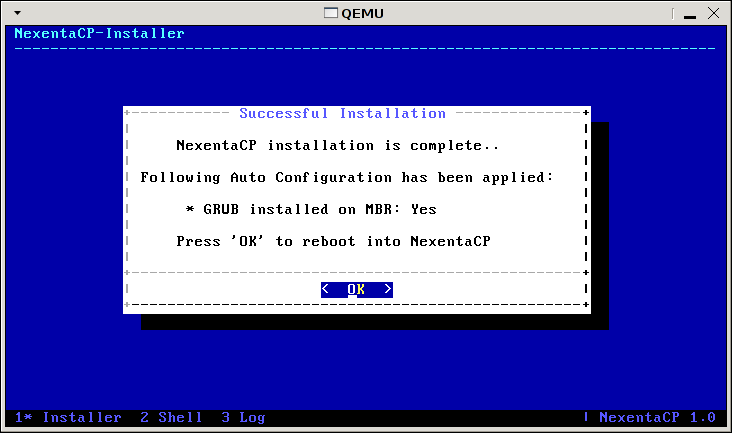
\includegraphics[width=0.5\hsize]{image200804/nexenta22.png}

\subsection{$B<B9T$7$F$_$k(B}

$B$=$l$G$O!"%$%s%9%H!<%k$7$?(BOS$B$r5/F0$7$F$_$^$7$g$&!#(B

\begin{commandline}
$ qemu-system-x86_64 -hda nexenta.cow \
 -m 512 -kernel-kqemu \
 -redir tcp:2299::22 \
 -nographic -serial stdio
\end{commandline}

$B<j85$N%7%9%F%`$G$O!"%3%^%s%I%i%$%s$G%m%0%$%s$,$G$-$k>uBV$^$G(B3$BJ,DxEY$+$+$j$^$7$?!#(B

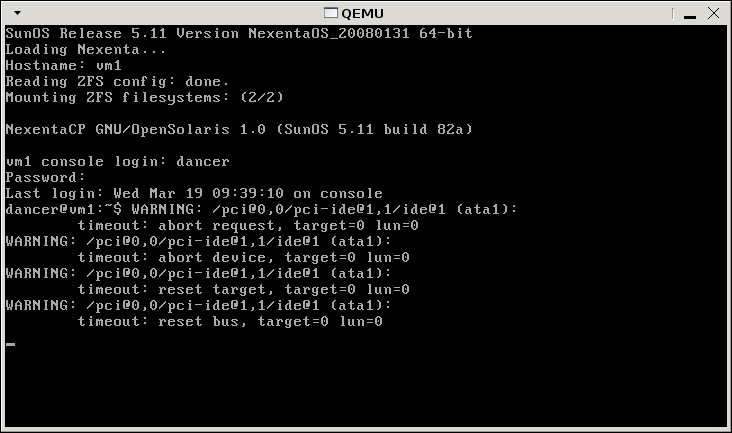
\includegraphics[width=0.5\hsize]{image200804/nexenta23.png}

$BDL>o$N%3%^%s%I%i%$%s%W%m%s%W%H$,N)$A>e$,$k$N$G!"%m%0%$%s$9$l$P$h$$$G$9!#(B

$B%G%U%)%k%H$G(B sshd \footnote{Debian $B$N%Q%C%1!<%8$H$O0[$J$j!"(BSUNWsshdu,
SUNWsshdr $B$J$I$N%Q%C%1!<%8$K$J$C$F$$$^$9!#8+$?46$8$O(B alien $B$G:n@.$5$l$F$$(B
$B$k%Q%C%1!<%8$N$h$&$G$9!#(B} $B$J$I$b%$%s%9%H!<%k$5$l$F$$$k$h$&$G$9!#(B
netstat $B$G3NG'$9$k$H(Blisten $B$7$F$$$k$h$&$G$9$N$G!"(Bssh $B$G%m%0%$%s$7$F:n6H(B
$B$9$k$3$H$,2DG=$J$h$&$G$9!#(B
$B$3$3$G$O!"(B qemu $B$G(B -redir $B%*%W%7%g%s$r;H$$!"(B SSH$B$N(B22$BHV%]!<%H$r%[%9%H(BOS$B$N(B
2299$B%]!<%H$+$i%"%/%;%9$G$-$k$h$&$K$7$F$$$^$9!#(B
$BLLE]$J$N$G!"(B -nographic -serial stdio $B%*%W%7%g%s$bDI2C$7$F%X%C%I%l%9$G2T(B
$BF/$5$;$F$_$^$9!#(B

$B%M%C%H%o!<%/%G%P%$%9$O(B ni0 $B$K$J$C$F$$$k$h$&$G$9!#(BIP$B%"%I%l%9$O(B qemu $B$N5!(B
$BG=$G(B DHCP$B$GDs6!$5$l$F$$$k%"%I%l%9!J(B10.0.2.15$B!K$K$J$C$F$$$^$9!#(B

\subsection{Debian $B$H$N8_49@-(B}

$B=i4|%$%s%9%H!<%k$N%Q%C%1!<%8?t$,Hs>o$KB?$$$G$9!#(BOpenSolaris $B$N%G%U%)%k%H(B
$B%$%s%9%H!<%k$KAjEv$9$k$b$N$r$=$N$^$^%Q%C%1!<%8$K$7$F$$$k$N$G$7$g$&$+!)(B
SUNW$B$G$O$8$^$k%Q%C%1!<%8L>$J$I$,$=$l$C$]$5$rJ*8l$j$^$9!#(B

\begin{commandline}
dancer@vm1:~$ dpkg -l | wc -l 
464
dancer@vm1:~$ dpkg -l 
Desired=Unknown/Install/Remove/Purge/Hold
| Status=Not/Installed/Config-files/Unpacked/Failed-config/Half-installed
|/ Err?=(none)/Hold/Reinst-required/X=both-problems (Status,Err: uppercase=bad)
||/ Name           Version        Description
+++-==============-==============-============================================
ii  adduser        3.80nexenta3   Add and remove users and groups
ii  alien          8.73.4         install non-native packages with dpkg
ii  apt            0.6.46.4nexent Advanced front-end for dpkg
ii  apt-utils      0.6.46.4nexent APT utility programs
ii  aptitude       0.4.4-1nexenta terminal-based apt frontend
[$BCfN,(B]
ii  sunw1394       5.11.82-1      Sun IEEE1394 Framework
ii  sunwaac        5.11.82-1      Adaptec AdvanceRaid Controller SCSI HBA Driv
ii  sunwad810      5.11.82-1      SUNW W1100z & W2100z Audio Drivers
ii  sunwadixp      5.11.82-1      SUNW Audio Driver for ATI IXP
ii  sunwadpu320    5.11.82-1      Adaptec Ultra320 Driver
ii  sunwafe        5.11.82-1      ADMtek Ethernet Driver
ii  sunwagp        5.11.82-1      AGP GART Driver
ii  sunwahci       5.11.82-1      Advanced Host Controller Interface (AHCI) SA
ii  sunwamd8111s   5.11.82-1      AMD8111 FAST Ethernet Network Adapter Driver
ii  sunwamr        5.11.82-1      LSI MegaRAID SCSI HBA Driver
[$BCfN,(B]
ii  sunwsshcu      5.11.82-1      SSH Common, (Usr)
ii  sunwsshdr      5.11.82-1      SSH Server, (Root)
ii  sunwsshdu      5.11.82-1      SSH Server, (Usr)
ii  sunwsshr       5.11.82-1      SSH Client and utilities, (Root)
ii  sunwsshu       5.11.82-1      SSH Client and utilities, (Usr)
ii  sunwtavor      5.11.82-1      Sun Tavor HCA driver
[$BN,(B]
\end{commandline}

\subsection{$B$J$$%Q%C%1!<%8$r%S%k%I$7$F$_$?(B}

/etc/hosts$B$r$$$8$C$F$_$h$&$H$7$?$i!"%7%s%\%j%C%/%j%s%/$K$J$C$F$^$7$?!#$7(B
$B$+$b(B root $B8"8B$G$b=q$-9~$_IT2D$K$J$C$F$$$^$9!#(B

\begin{commandline}
root@vm1:/export/home/dancer# ls -l /etc/hosts
lrwxrwxrwx 1 root root 12 Mar 19 08:15 /etc/hosts -> ./inet/hosts
root@vm1:/export/home/dancer# ls -l /etc/inet/hosts -l 
-r--r--r-- 1 root sys 1078 Apr  6 10:28 /etc/inet/hosts
\end{commandline}

$B5$$r$H$j$J$*$7$F!"(B /etc/apt/sources.list $B$KE,Ev$K%=!<%9$rDI2C$7$^$9!#(B

\begin{commandline}
deb-src http://cdn.debian.or.jp/debian unstable main contrib non-free
\end{commandline}

apt-listbugs $B$,B8:_$7$J$$$_$?$$$J$N$G!"%S%k%I$7$F$_$h$&$H;W$$$^$9!#(B

$B$^$:!"$J$<$@$+(B racc, rdtool $B$,B-$j$J$$$N$G%S%k%I$7$F%$%s%9%H!<%k$7$^$9!#(B
$BL5;v$K(Bapt-listbugs $B<+BN$b%S%k%I$G$-$?$N$G!"0U5$MH!9$H%$%s%9%H!<%k$7$F$_$^(B
$B$9!#(B

\begin{commandline}
root@vm1:/tmp/apt-listbugs-0.0.88# debi
Selecting previously deselected package apt-listbugs.
(Reading database ... 27441 files and directories currently installed.)
Unpacking apt-listbugs (from apt-listbugs_0.0.88_all.deb) ...
dpkg: dependency problems prevent configuration of apt-listbugs:
 apt-listbugs depends on ruby (>= 1.8); however:
  Package ruby is not installed.
 apt-listbugs depends on libruby1.8 (>= 1.8.5); however:
  Version of libruby1.8 on system is 1.8.4-1nexenta1.3.
 apt-listbugs depends on libdpkg-ruby1.8 (>= 0.3.2); however:
  Package libdpkg-ruby1.8 is not installed.
 apt-listbugs depends on libgettext-ruby1.8; however:
  Package libgettext-ruby1.8 is not installed.
 apt-listbugs depends on libxml-parser-ruby1.8; however:
  Package libxml-parser-ruby1.8 is not installed.
 apt-listbugs depends on libhttp-access2-ruby1.8 (>= 2.0.6); however:
  Package libhttp-access2-ruby1.8 is not installed.
dpkg: error processing apt-listbugs (--install):
 dependency problems - leaving unconfigured
Errors were encountered while processing:
 apt-listbugs
debi: debpkg -i failed
\end{commandline}

$B;DG0!"$$$/$D$+%(%i!<$,$"$k$h$&$G$9!#(Bruby $B<+BN$,8E$$$H$$$&%(%i!<$d!"$$$/$D(B
$B$+$N%i%$%V%i%j$,B-$j$J$$$H$$$&%(%i!<$,$G$F$$$^$9!#(B

$B2r7h$G$-$=$&$JLdBj$b!"2r7h$G$-$J$5$=$&$JLdBj$b$"$j$^$9!#@h$OD9$$$+!)(B

\subsection{$B:#8e$NE8K>!)(B}


\clearpage

%\printindex

\cleartooddpage

\vspace*{15cm}
\hrule
\vspace{2mm}

\includegraphics[width=2cm]{image200502/openlogo-nd.eps}
\noindent \Large \bf Debian $BJY6/2q;qNA(B\\ \\
\noindent \normalfont \debmtgyear{}$BG/(B\debmtgmonth{}$B7n(B\debmtgdate{}$BF|(B \hspace{5mm}  $B=iHGBh(B1$B:~H/9T(B\\
\noindent \normalfont $BEl5~%(%j%"(B Debian $BJY6/2q(B $B!JJT=8!&0u:~!&H/9T!K(B\\
\hrule


\end{document}
